%\newpage
\section{Functional View}

A deep neural network can be seen as a family of parametric, non-linear, and hierarchical representation learning functions. These learning functions are massively optimized with stochastic gradient descent (SGD) over some pre-specified objectives, such as the loss of a set of training instances. It is expected that, the learned functions will encode domain knowledge that is implicitly presented in the training instances. 


\subsection{Mappings between High-dimensional Spaces}

Consider a feed-forward network as shown in Figure~\ref{fig:feedforward}. Assume that it has $m+1$ layers, where Layer-0 is the input layer,  Layer-$m$ is the output layer, and Layer-1 to Layer-$(m-1)$ are the hidden layers. 

\begin{figure}[!htbp]
    \centering
    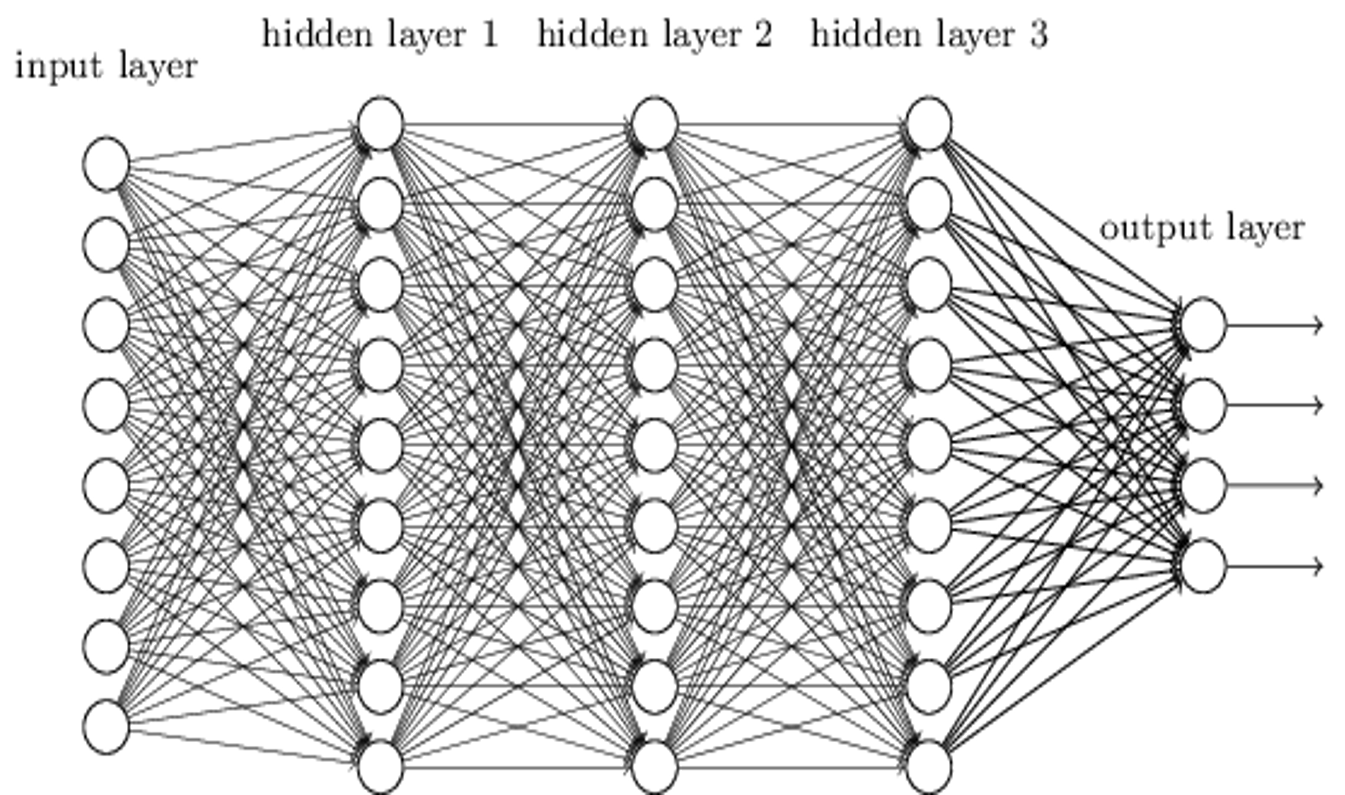
\includegraphics[width=0.6\textwidth]{images/deepLearning/functionalView/nn.png}
    \caption{A 5 layer feed-forward network}
    \label{fig:feedforward}
\end{figure}

Every layer is a function, so we have functions $f_1,...,f_{m}$, for hidden layers and output layer, and because every function is parameterised, we use $\textbf{W}=\{\textbf{W}_1,...,\textbf{W}_m\}$ to denote their parameters. Based on these, a neural network can be written in a functional way as follows. 

\begin{equation}
    f_{\textbf{W}}(\textbf{x};\textbf{W}_1,...,\textbf{W}_m) = f_m(f_{m-1}(... f_1(\textbf{x};\textbf{W}_1),\textbf{W}_{m-1});\textbf{W}_m)
\end{equation}
Alternatively, we may write 
\begin{equation}\label{equ:mappings}
\begin{array}{lclcl}
    f_{\textbf{W}}(\textbf{x}) & = & \textbf{v}_m & = &  f_{m}(\textbf{v}_{m-1};\textbf{W}_{m})\\
   && \textbf{v}_{m-1} & = & f_{m-1}(\textbf{v}_{m-2};\textbf{W}_{m-1}) \\
   && ...\\
   && \textbf{v}_{2} & = & f_{2}(\textbf{v}_{1};\textbf{W}_{2}) \\
   && \textbf{v}_{1} & = & f_{1}(\textbf{v}_{0};\textbf{W}_{1}) \\
\end{array}
\end{equation}
where $\textbf{v}_i$ is the output value of Layer-$i$. Note that, we have both $\textbf{v}_i$ and $\textbf{W}_i$ as vectors or matrices, because it is typical that there are many neurons per layer and the layer functions are parameterised with many parameters. 

Take a closer look at Equation (\ref{equ:mappings}), given a function $\textbf{v}_{i} = f_{i}(\textbf{v}_{i-1};\textbf{W}_{i})$, once the parameters $\textbf{W}_i$ are learned, it is a transformation from $\textbf{v}_{i-1}$ to $\textbf{v}_{i}$. Let each layer-$i$ have $k_i$ neurons, we have that  $\textbf{v}_{i-1}$ is a vector of $k_{i-1}$ entries and $\textbf{v}_{i}$ is a vector of $k_{i}$ entries. Therefore, the transformation can be seen as a mapping from high-dimensional space $\real^{k_{i-1}}$ to $\real^{k_{i}}$. Generalise this to the entire network, we have 
\begin{equation}
   \displaystyle \real^{k_0} \xmapsto{f_1} \real^{k_1} \xmapsto{f_2} ... \xmapsto{f_m} \real^{k_m}
\end{equation}
Note that, $k_0$ is the number of input features and $k_m$ is the number of class labels. 

\subsection*{Training Objective}

The training typically intends to get the best weights $\textbf{W}^*$ as follows. 
\begin{equation}
    \textbf{W}^* \leftarrow \argmin_{\textbf{W}} \sum_{(\textbf{x},{y})\in D} L(y,\textbf{v}_m)
\end{equation}
where $L(y,f_{\textbf{W}}(\textbf{x}))$ is typically a loss function measuring the gap between actual label $y$ with its current prediction $f_{\textbf{W}}(\textbf{x})$. 
However, the optimisation problem is highly dimensional and non-convex. Therefore, in most cases, the training ends up with an approximation $\hat{\textbf{W}}$. 

\subsection{Recurrent Neural Networks}

The above is mainly for feedforward neural networks (FNNs), which model a function $\dnnfunction:X\rightarrow Y$ that maps from input domain $X$ to output domain $Y$: given an input $x\in X$, it outputs the prediction $y\in Y$. For a sequence of inputs $x_1,\dots,x_n$, an FNN $\dnnfunction$ considers each input individually, that is, $\dnnfunction(x_i)$ is independent from $\dnnfunction(x_{i+1})$. 

%and is %usually 
%used to perform predictions based on an input $x\in X$, or recognise patterns in $x$. 
%For a sequence of inputs $x_1,...,x_n$, $\dnnfunction$ will handle them individually without considering  results from previous predictions, that is, the result of $\dnnfunction(x_i)$ is independent of the results of $\dnnfunction(x_j)$ when $j\neq i$. 

By contrast, a recurrent neural network (RNN) 
%are designed to handle sequential data. An RNN contains at least one recurrent layer
%, as depicted in Fig.~\ref{fig:recurrent}, 
%that 
processes 
an input sequence by iteratively taking inputs one by one. 
%sequential input.
%illustrates how a sequential input is handled by a recurrent layer by unfolding.
A recurrent layer can be modeled as a function 
$\rnnfunction:X'\times C\times Y' \rightarrow C\times Y'$
such that 
$\rnnfunction(x_t,c_{t-1},h_{t-1})=(c_t,h_t)$ for $t=1,...,n$, 
where $t$ denotes the $t$-th time step, $c_t$ is the cell state used to represent the intermediate memory and $h_{t}$ is the output of the $t$-th time step.  
More specifically, the recurrent layer takes three inputs: $x_t$ at the current time step, the prior memory state $c_{t-1}$ and the prior cell output $h_{t-1}$; consequently, it updates the current cell state $c_t$ and outputs current $h_{t}$.   
%Initially, we let $c_0$ and $h_0$ be 0-valued vectors. For a (finite) sequence of inputs $x_1,...,x_n$, this function $\rnnfunction$ is applied recursively on them. 
%For example, the popular long short-term memory (LSTM) layer can be represented with the following equations for time~$t$: 

RNNs differ from each other given their respective definitions, i.e., internal structures, of recurrent layer function $\rnnfunction$, of which long short-term memory (LSTM) in Equation (\ref{eq:lstm}) is the most popular and commonly used one. 
%
\begin{equation}
\label{eq:lstm}
\begin{array}{lcl}
f_t & = & \sigma(W_f\cdot [h_{t-1},x_t] + b_f) \\ 
i_t & = & \sigma(W_i\cdot [h_{t-1},x_t] + b_i) \\ 
c_t & = & f_t*c_{t-1} + i_t * \tanh(W_c\cdot [h_{t-1},x_t] + b_c)\\
o_t & = & \sigma(W_o\cdot [h_{t-1},x_t] + b_o) \\ 
h_t & = &  o_t * \tanh(c_t)
\end{array}
\end{equation}
%
such that $\sigma(x)\in [0,1]$ for any $x\in\real$, $\tanh$ is the hyperbolic tangent function such that $\tanh(x)\in [-1,1]$ for any $x\in\mathbb{R}$, $W_f,W_i,W_c,W_o$ are weight matrices, $b_f,b_i,b_c,b_o$ are bias vectors,  $f_t,i_t,o_t$ are internal gate variables, $h_t$ is the hidden state variable (utilising $o_t$), and $c_t$ is the cell state variable. For the connection with successive layers, we only take the last output $h_n$ as the output. For simplicity, when working with finite sequential data, we can also define a recurrent layer as $\rnnfunction:(X')^n\rightarrow Y'$, which takes, as input, a sequential data of length $n$ and returns the last output $h_n$. Figure~\ref{fig:Cell} presents an illustrative diagram for LSTM cell. 

\begin{figure}[!htbp]
    \centering
    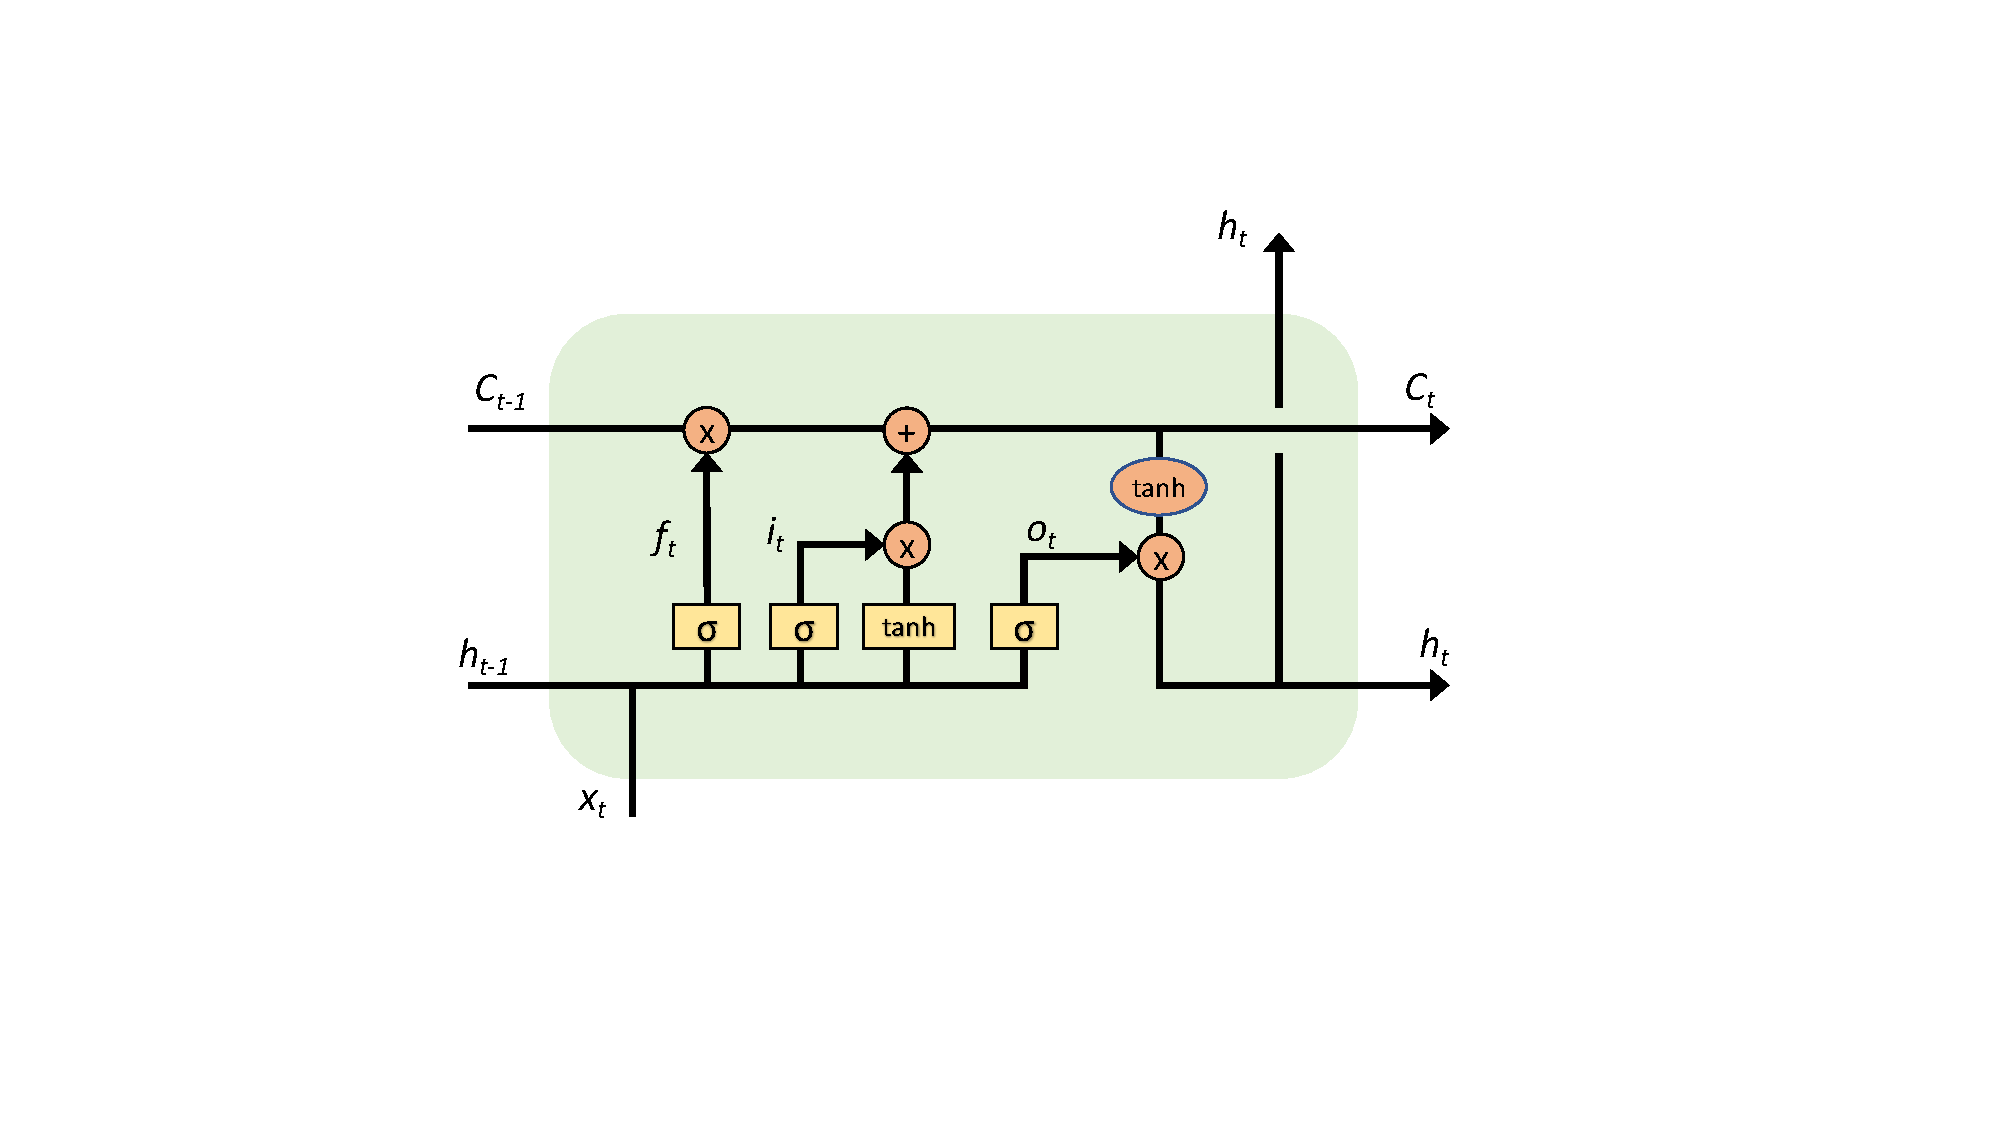
\includegraphics[width=0.65\linewidth]{images/deepLearning/functionalView/LSTM_cell.pdf}
    \caption{LSTM Cell}
    \label{fig:Cell}
\end{figure}


In LSTM, $\sigma$ is the sigmoid function and $\tanh$ is the hyperbolic tangent function; $W$ and $b$ represent the weight matrix and bias vector, respectively; $f_t,i_t,o_t$ are internal gate variables of the cell.
%Fig. \ref{fig:Cell} gives an diagrammatic illustration of an LSTM cell. 
In general, the recurrent layer (or LSTM layer) is connected to non-recurrent layers such as fully connected layers so that the cell output propagates further. We denote the remaining layers with a function $\dnnfunction_2:Y'\rightarrow Y$. Meanwhile, there can be feedforward layers connecting to the RNN layer, and we let it be another function $\dnnfunction_1:X\rightarrow X'$. As a result, the RNN model that accepts a sequence of inputs $x_1,\dots,x_n$ can be modeled as a function $\varphi$ such that 
%\begin{equation}
$\varphi(x_1...x_n) = \dnnfunction_2\cdot\rnnfunction(\prod_{i=1}^n \dnnfunction_1(x_i))$.
%\end{equation}
%
%
Normally, the recurrent layer is connected to non-RNN layers such as fully connected layers so that the output $h_n$ is processed further. We let the remaining layer be a function $\dnnfunction_2:Y'\rightarrow Y$. Moreover, there can be feedforward layers connecting to the RNN layer, and we let it be a function $\dnnfunction_1:X\rightarrow X'$. Then given a sequential input $x_1,...,x_n$, the RNN is a function $\varphi$ such that 
%



\subsection{Learning Representation and Features}\label{sec:representationlearning}

\subsection*{Raw digital representation}

Every instance has to be represented in a digital form. For example, the 8th instance in the \textbf{digits} dataset is an image of digit 8 as shown in Figure~\ref{fig:digit8}. 

\begin{figure}[!htbp]
    \centering
    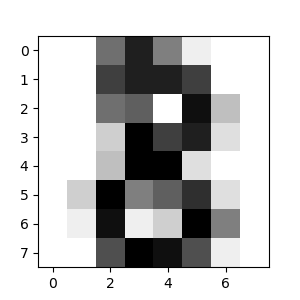
\includegraphics[width=0.2\textwidth]{images/deepLearning/functionalView/digit_8.png}
    \caption{A small image of digit 8}
    \label{fig:digit8}
\end{figure}

Actually, it is stored as a matrix as follows:  

\begin{equation}
\begin{blockarray}{cccccccc}
\begin{block}{(cccccccc)}
0 &   0 &   9 &  14 &   8 &   1 &   0 &   0 \\
0 &   0 &  12 &  14 &  14 &  12 &   0 &   0 \\
0 &   0 &   9 &  10 &   0 &  15 &   4 &   0 \\
0 &   0 &   3 &  16 &  12 &  14 &   2 &   0 \\
0 &   0 &   4 &  16 &  16 &   2 &   0 &   0 \\
0 &   3 &  16 &   8 &  10 &  13 &   2 &   0 \\
0 &   1 &  15 &   1 &   3 &  16 &   8 &   0 \\
0 &   0 &  11 &  16 &  15 &  11 &   1 &   0  \\
\end{block}
\end{blockarray}
\end{equation}

As another example, the videos are actually a sequence of images, and therefore it is stored as a 3-dimensional array. 

Features are domain dependent. Evidently, for computer vision, pixels are input features, and for natural language processing, words are input features. In addition to input features which closely relate to data representation, we may use the term latent features or hidden features for those features in the hidden layers. 

\subsection*{Feature Extraction}

is one of the key intermediate tasks for learning, for both traditional machine learning and deep learning. It is a process that identifies important features or attributes of the data.  For traditional machine learning, as shown in Figure~\ref{fig:traditionalMLflow}, it first extracts features and then applies a learnable classifier.  
\begin{figure}[!htbp]
    \centering
    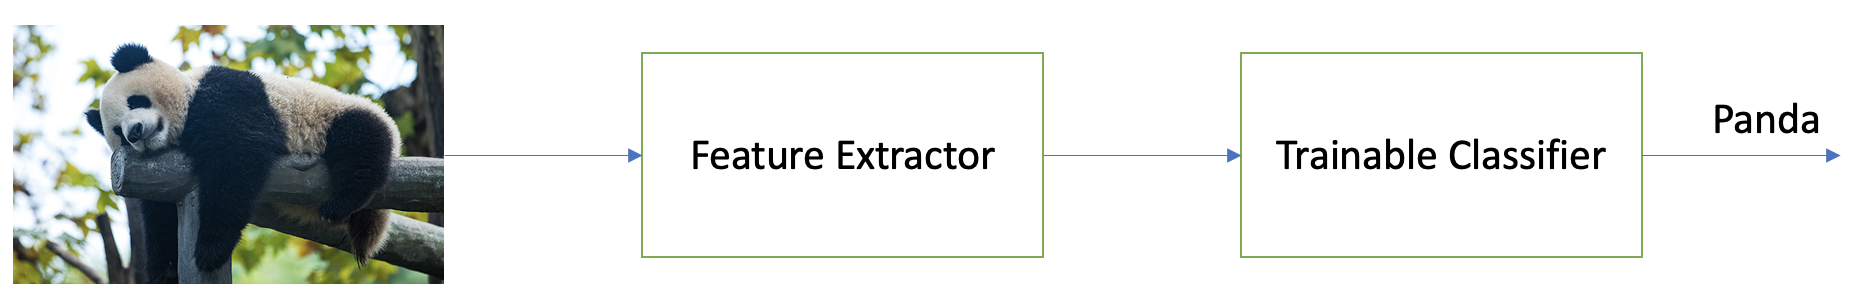
\includegraphics[width=0.9\textwidth]{images/deepLearning/functionalView/traditionalML.png}
    \caption{Flow of traditional machine learning}
    \label{fig:traditionalMLflow}
\end{figure}
The feature extraction is treated as a step independent of the classification. There are many different methods for feature extraction, for example, SIFT (scale-invariant feature transform). 

Deep learning, however, requires only one step (i.e., end-to-end) to implement both feature extraction and classification, as shown in Figure~\ref{fig:deeplearningflow}. 
\begin{figure}[!htbp]
    \centering
    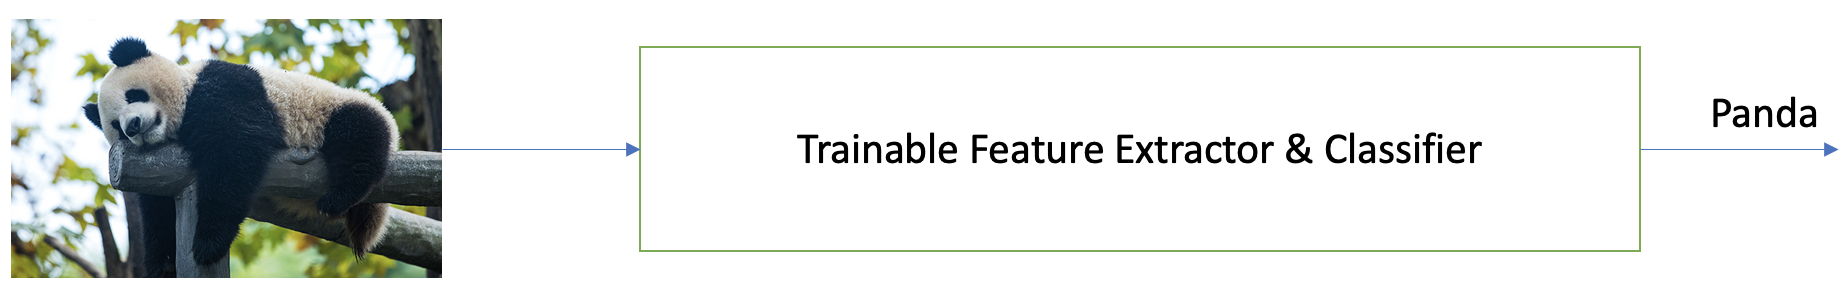
\includegraphics[width=0.9\textwidth]{images/deepLearning/functionalView/deeplearningflow.png}
    \caption{Flow of deep learning}
    \label{fig:deeplearningflow}
\end{figure}
Both the feature extractor and the classifier are trained at the same time. 

Feature extraction is closely related to dimensionality reduction, i.e., to separate data as much as possible. Most data distributions and tasks are non-linear, so a linear assumption is often convenient, but not necessarily truthful. Therefore, to get non-linear machines without too much effort, we may have to consider non-linear features. 

There are many ways to get non-linear features, including e.g., 
\begin{itemize}
    \item application of non-linear kernels, e.g., polynomial, RBF, etc.
    \item explicit design of features, e.g., SIFT, HOG, etc. 
\end{itemize}

The quality of features is usually evaluated against  the following few criteria: 
\begin{itemize}
    \item invariance
    \item repeatabilty 
    \item discriminativeness  
    \item robustness 
\end{itemize}
It is useful to note that these criteria may be conflicting. Hence, there needs to be a trade-off between criteria. 

\subsection*{Data manifold}

Actually, most natural, high-dimensional data (e.g. faces) lie on lower dimensional manifolds. For example, Figure~\ref{fig:swissRoll} is the so-called ``swiss roll'', where the data points are 3-dimensional, but they all lie on a 2-dimensional manifold. That is, the actual dimensionality of the manifold is 2, while the dimensionality of the input space is 3. 


\begin{figure}[!htbp]
    \centering
    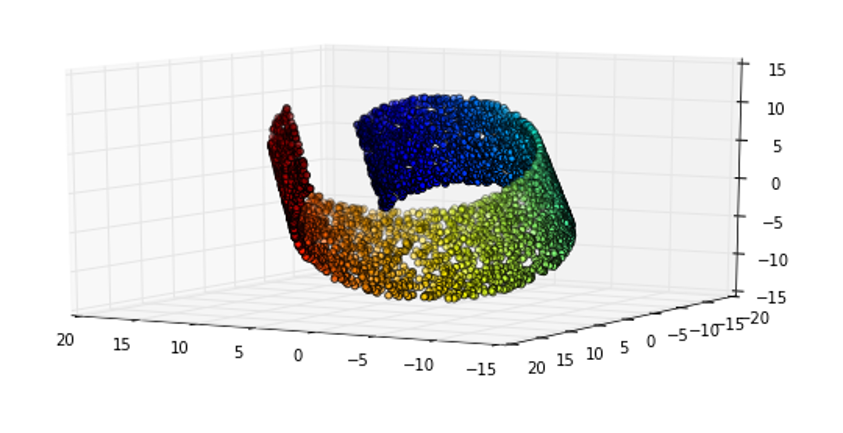
\includegraphics[width=0.7\textwidth]{images/deepLearning/functionalView/swissRoll.png}
    \caption{Data manifold -- ``swiss role'' example}
    \label{fig:swissRoll}
\end{figure}

Therefore, although the data points may consist of thousands of features, they can be described as a function of only a few underlying parameters. That is, the data points are actually sampled from a low-dimensional manifold that is embedded in a high-dimensional space. 

\subsection*{Difficulties of simply using dimensionality reduction or kernel}


The above observation suggests that our goal should be on discovering lower dimensional manifolds. We remark that, these manifolds are most probably highly non-linear. 

The success of this requires two hypotheses: 

\begin{itemize}
    \item If we can compute the coordinates of the input (e.g., a face image) to this non-linear manifold then the data become separable. This hypothesis suggests the existence of \emph{functional mapping}. For the ``swiss role'' example, there should be a (non-linear) function mapping from 3d space to 2d space, on which the data can be linearly separable.
    \item Semantically similar things lie closer than semantically dissimilar things. This implies the existence of applicable dimensional reduction methods. 
\end{itemize}







While raw data live in huge dimensionality, semantically meaningful raw data prefer lower dimensional manifolds, which still live in the same huge dimensionality. 
Can we discover this manifold to embed our data on? 


\subsection*{End-to-end learning of feature hierarchies}

The above discussions basically suggest that, it is an almost impossible task to manually craft features and also nontrivial to design algorithms (dimensionality reduction, functional mapping, etc) to compute features. This is in stark contrast with deep learning. Actually, one of the key advantages of convolutional neural networks is their ability to learn (or extract) features automatically.  

In a CNN, there are a pipeline of successive layers, such that each layer’s output is the input for the next layer. 
Layers produce features of higher and higher abstractions, such that the shadow layers extract low-level features (e.g. edges or corners), middle layers extract mid-level features (e.g. circles, squares, textures), and deep layers capture high level, class-specific features (e.g. face detector). See Figure~\ref{fig:featureVisualisation}. 

\begin{figure}[!htbp]
    \centering
    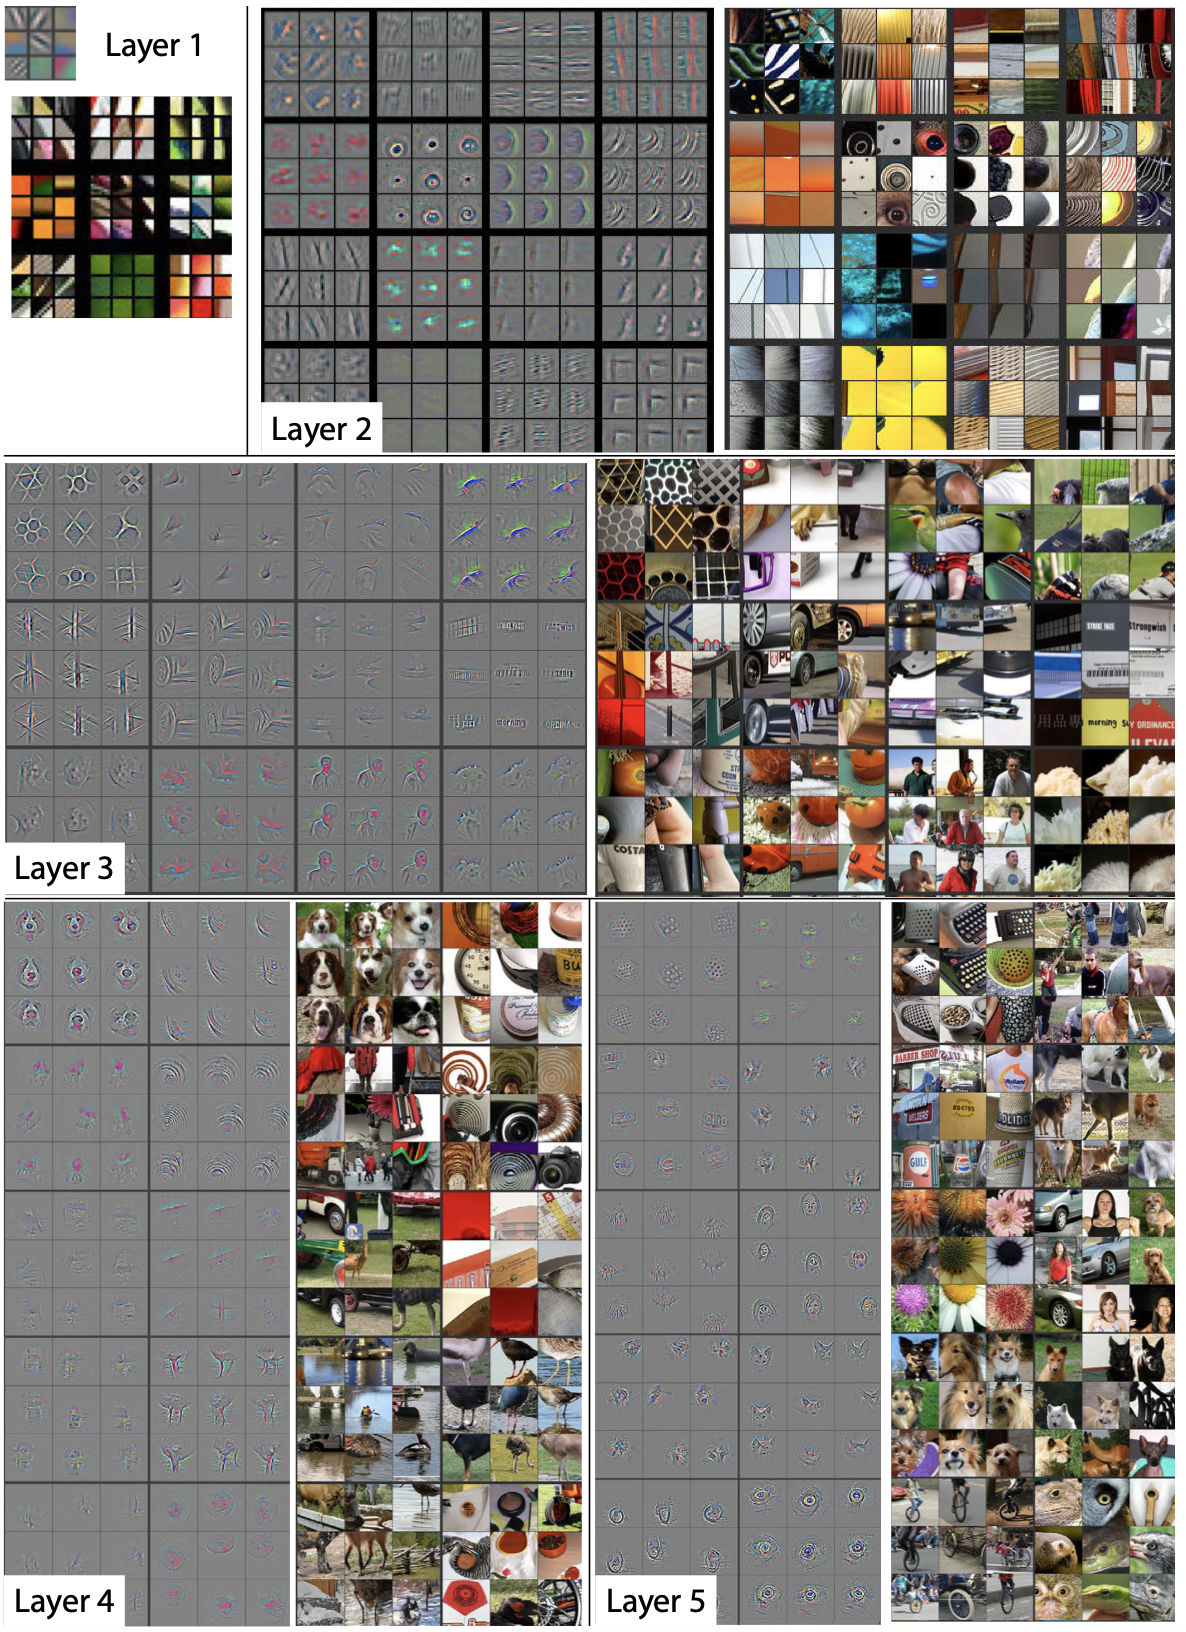
\includegraphics[width=\textwidth]{images/deepLearning/functionalView/featureVisualisation.png}
    \caption{Visualisation of features in hidden layers  \cite{DBLP:journals/corr/ZeilerF13}}
    \label{fig:featureVisualisation}
\end{figure}

We remark that, for CNNs, it has been shown that, preferably, training data should be as raw as possible. That is, no additional feature extraction phase  is needed. 



\subsection*{Why learn the features?}

Manually designed features 
often take a lot of time to come up with and implement, a lot of time to validate, and are incomplete, as one cannot know if they are optimal for the task. 
%
On the other hand, learned features 
are easy to adapt,  
very compact and specific to the task at hand. 
Given a basic architecture in mind, it is relatively easy and fast to optimize, i.e., 
time spent on designing features is now spent on designing architectures. 

\newpage
\subsection{Practice}

The following is a code to train a neural network with fully-connected layers. 

\subsection*{Train a fully connected model}

First of all, we install two packages torch and torchvision.

\begin{cmds}
pip3 install torch
pip3 install torchvision
\end{cmds}

Then, we set up hyper-parameters (e.g., batchsize, epoch, learning rate), device (e.g., CPU or GPU), and load training dataset (MNIST). 

\begin{lstlisting}[language=Python]
import torch
import torch.nn as nn
import torch.nn.functional as F
import torch.optim as optim
from torchvision import datasets, transforms
import argparse
import time

# Setup hyper-parameter
parser = argparse.ArgumentParser(description='PyTorch MNIST Training')
parser.add_argument('--batch-size', type=int, default=128, metavar='N',
                    help='input batch size for training (default: 128)')
parser.add_argument('--test-batch-size', type=int, default=128, metavar='N',
                    help='input batch size for testing (default: 128)')
parser.add_argument('--epochs', type=int, default=10, metavar='N',
                    help='number of epochs to train')
parser.add_argument('--lr', type=float, default=0.01, metavar='LR',
                    help='learning rate')
parser.add_argument('--no-cuda', action='store_true', default=False,
                    help='disables CUDA training')
parser.add_argument('--seed', type=int, default=1, metavar='S',
                    help='random seed (default: 1)')

args = parser.parse_args(args=[]) 

# Judge cuda is available or not
use_cuda = not args.no_cuda and torch.cuda.is_available()
#device = torch.device("cuda" if use_cuda else "cpu")
device = torch.device("cpu")

torch.manual_seed(args.seed)
kwargs = {'num_workers': 1, 'pin_memory': True} if use_cuda else {}

# Setup data loader
transform=transforms.Compose([
        transforms.ToTensor(),
        transforms.Normalize((0.1307,), (0.3081,))
        ])
trainset = datasets.MNIST('../data', train=True, download=True,
                   transform=transform)
testset = datasets.MNIST('../data', train=False,
                   transform=transform)
train_loader = torch.utils.data.DataLoader(trainset,batch_size=args.batch_size, shuffle=True,**kwargs)
test_loader = torch.utils.data.DataLoader(testset,batch_size=args.test_batch_size, shuffle=False, **kwargs)
\end{lstlisting}

We can define a fully connected network as follows, with the structure 784-128-64-32-10,

\begin{lstlisting}[language=Python]
# Define fully connected network
class Net(nn.Module):
    def __init__(self):
        super(Net, self).__init__()
        self.fc1 = nn.Linear(28*28, 128)
        self.fc2 = nn.Linear(128, 64)
        self.fc3 = nn.Linear(64, 32)
        self.fc4 = nn.Linear(32, 10)

    def forward(self, x):
        x = self.fc1(x)
        x = F.relu(x)
        x = self.fc2(x)
        x = F.relu(x)
        x = self.fc3(x)
        x = F.relu(x)
        x = self.fc4(x)
        output = F.log_softmax(x, dim=1)
        return output
\end{lstlisting}

Then, we define the training function, which computes loss and updates parameters for each minibatch. 

\begin{lstlisting}[language=Python]
# Training function
def train(args, model, device, train_loader, optimizer, epoch):
    model.train()
    for batch_idx, (data, target) in enumerate(train_loader):
        data, target = data.to(device), target.to(device)
        data = data.view(data.size(0),28*28)
        
        # Clear gradients
        optimizer.zero_grad()
        
        # Compute loss
        loss = F.cross_entropy(model(data), target)
        
        # Get gradients and update
        loss.backward()
        optimizer.step()
\end{lstlisting}

We also can define a predict function, which outputs training loss and test loss for each epoch. 

\begin{lstlisting}[language=Python]
# Predict function
def eval_test(model, device, test_loader):
    model.eval()
    test_loss = 0
    correct = 0
    with torch.no_grad():
        for data, target in test_loader:
            data, target = data.to(device), target.to(device)
            data = data.view(data.size(0),28*28)
            output = model(data)
            test_loss += F.cross_entropy(output, target, size_average=False).item()
            pred = output.max(1, keepdim=True)[1]
            correct += pred.eq(target.view_as(pred)).sum().item()
    test_loss /= len(test_loader.dataset)
    test_accuracy = correct / len(test_loader.dataset)
    return test_loss, test_accuracy
\end{lstlisting}

Finally, we define the main function and call the training function for each epoch.

\begin{lstlisting}[language=Python]
# Main function, train the dataset and print training loss, test loss
def main():
    model = Net().to(device)
    optimizer = optim.SGD(model.parameters(), lr=args.lr)
    for epoch in range(1, args.epochs + 1):
        start_time = time.time()
        
        # Training
        train(args, model, device, train_loader, optimizer, epoch)
        
        # Get trnloss and testloss
        trnloss, trnacc = eval_test(model, device, train_loader)
        tstloss, tstacc = eval_test(model, device, test_loader)
        
        # Print trnloss and testloss
        print('Epoch '+str(epoch)+': '+str(int(time.time()-start_time))+'s', end=', ')
        print('trn_loss: {:.4f}, trn_acc: {:.2f}%'.format(trnloss, 100. * trnacc), end=', ')
        print('test_loss: {:.4f}, test_acc: {:.2f}%'.format(tstloss, 100. * tstacc))

if __name__ == '__main__':
    main()
\end{lstlisting}
